\section{Positive Definite Graphs}

As another example of the symmetric matrix $C$ from above, consider
$I_2(m)$:
\[
C = \begin{pmatrix}
    2 & -2 \cos \frac{\pi}{m} \\
    -2 \cos \frac{\pi}{m} & 2
\end{pmatrix}
\]

Note that if $s_\alpha, s_\beta \in S$ are the reflections in the hyperplanes
$H_\alpha, H_\beta$ in an Euclidean space $V$, and $||\alpha|| = ||\beta|| =
\sqrt{2}$ then
\begin{align*}
    (\alpha, \beta) &= ||\alpha|| \cdot ||\beta|| \cdot \cos \phi \\
    &= 2 \cos \left( \frac{m_{\alpha \beta}-1}{m_{\alpha \beta}} \pi \right) \\
    &= -2 \cos \left( \frac{\pi}{m_{\alpha \beta}} \right)
\end{align*}
(Recall \S 1.3, where we showed the simple reflections in $I_2(m)$ meet at an
angle of $\frac{\pi}{m}$.)

The $r \times r$ matrix $C$, as well as the corresponding Coxeter graph,
are called {\em positive definite} if
\[
    \sum_{i, j} x_i C_{ij} x_j > 0
\]
for all nonzero $x \in \R^r$. There are various characterisations of positive
definite symmetric real matrices $A$:
\begin{enumerate}
\item[(1)] All its eigenvalues are positive (and real).
\item[(2)] All its principal minors are positive (Sylvester's criterion).
\item[(3)] $(x, y) := \sum_{i,j} x_i A_{ij} y_j$ ($x,y \in \R^r$) is an inner product.
\end{enumerate}

Note: if $A = (a_{ij})$ is an $r \times r$ matrix,
%\[
%    A = \begin{pmatrix}
%        a_{11} & \dots & a_{1r} \\
%        \vdots & \ddots & \vdots \\
%        a_{r1} & \dots & a_{rr}
%    \end{pmatrix},
%\]
then the $k^{\text{th}}$ (or possibly $(r-k)^{\text{th}}$)
principal minor, for $1 \leq k \leq r$, is
\[
    \det \begin{pmatrix}
        a_{11} & \dots & a_{1k} \\
        \vdots & \ddots & \vdots \\
        a_{k1} & \dots & a_{kk}
    \end{pmatrix}.
\]

This last characterisation is particularly relevant for us since we are dealing
with finite reflection groups for which (3) holds by construction. It is our
usual positive definite bilinear symmetric form on $V$.
Moreover $C_{\alpha \beta} = (\alpha, \beta)$ provided we normalise all simple
roots as $||\alpha|| = \sqrt{2}$.

Hence, we need to classify all positive definite real symmetric matrices.
Our strategy will be to identify graphs
to act as a `boundary' on the space of positive definite graphs, intuitively
replacing the condition $>0$ with $\geq 0$.

Before we do this, we list a collection of graphs that are not positive definite.

\begin{lemma} \label{lem15}
The following graphs are {\em not} positive definite.
\end{lemma}

\begin{center}
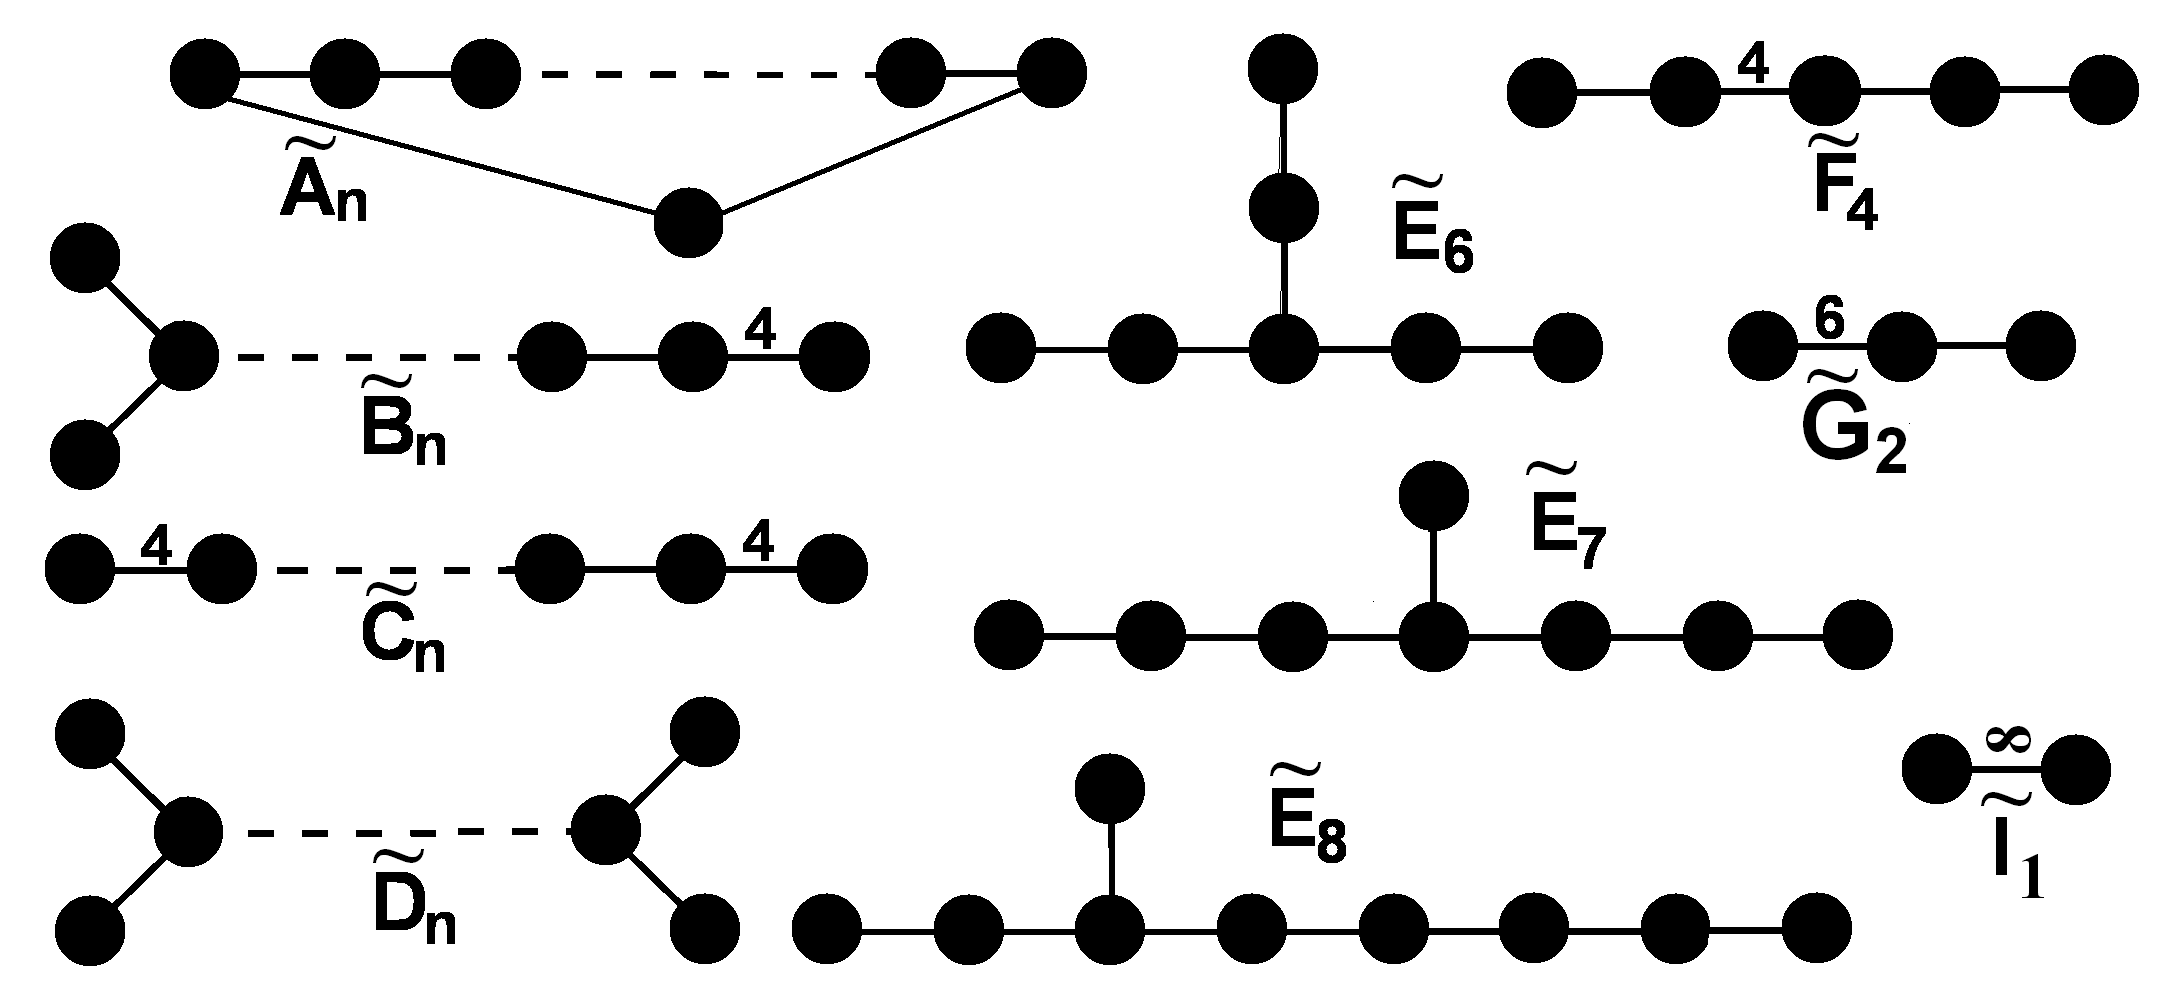
\includegraphics[width=0.7\textwidth]{img/affine-groups.png}

\begin{picture}(3,0.7)
\put(0,0.2){\circle*{0.2}}
\put(0,0.2){\line(1,0){1}}
\put(1,0.2){\circle*{0.2}}
\put(1,0.2){\line(1,0){1}}
\put(2,0.2){\circle*{0.2}}
\put(2,0.2){\line(1,0){1}}
\put(3,0.2){\circle*{0.2}}
\put(1.4,0.3){$5$}
\end{picture}

\begin{picture}(4,0.7)
\put(0,0.2){\circle*{0.2}}
\put(0,0.2){\line(1,0){1}}
\put(1,0.2){\circle*{0.2}}
\put(1,0.2){\line(1,0){1}}
\put(2,0.2){\circle*{0.2}}
\put(2,0.2){\line(1,0){1}}
\put(3,0.2){\circle*{0.2}}
\put(3,0.2){\line(1,0){1}}
\put(4,0.2){\circle*{0.2}}
\put(3.4,0.3){$5$}
\end{picture}
\end{center}

(Image courtesy of Wikipedia. The final two are of `hyperbolic type'.)
We will denote $\widetilde{A}_1 =
\widetilde{I}_1$, $\widetilde{B}_2 = \widetilde{C}_2$. Note that
$\widetilde{A}_n$, $\widetilde{B}_n$, $\widetilde{C}_n$, $\widetilde{D}_n$
contain $n+1$ vertices.
These four cases must be checked for all $n$, the rest can be directly
checked.

\begin{proof}
For all of the graphs of type $\widetilde{G}$ (affine type) we claim that $\det
(C_{\widetilde{G}}) = 0$.

In each case this is an elementary exercise, and we only consider a few examples:

For $\widetilde{A}_{n-1}$, we have
\[
    C = \begin{pmatrix}
        2 & -1 & 0 & \cdots & -1 \\
        -1 & 2 & -1 & \cdots & 0 \\
        0 & -1 & 2 & & \vdots \\
        \vdots & \vdots & & \ddots & -1 \\
        -1 & 0 & \cdots & -1 & 2
    \end{pmatrix}
\]
and since the sum of the rows is zero, so the determinant is zero.
Note that for an arbitrary $n \times n$ circulant matrix, i.e. one which can
be determined by shifts of its first column, with first column given by
$(c_0, c_1, \dots, c_{n-1})^t$, we have
\[
    \det C = \prod_{k=0}^{n-1} \sum_{j=0}^{n-1} c_j e^{\frac{2\pi i \cdot jk}{n}}.
\]
For us, $c_0 = 2$, $c_1 = c_{n-1} = -1$, and other $c_i = 0$, so
\[
    \det C = \prod_{k=0}^{n-1} \left(2-2 \cos \frac{2 \pi k}{n}\right) = 0.
\]
\end{proof}
